\documentclass[a4paper,11pt]{article}

\usepackage{estiloBase}
\usepackage{colores}
\usepackage{bera}
\usepackage{comandos}


\def \titulo{oFlute: blablablá título largo}
\def \autor{Alumno: José Tomás Tocino García\\Tutores: Manuel Palomo Duarte, Antonio García Domínguez}
\def \fecha{Agosto de 2010}

%\margenes

% Directorio de imágenes
%\graphicspath{{../img/}}

\begin{document}
\portada

\abstract{\textbf{oFlute} se modela como una herramienta lúdico-educativa para
  alumnos que comiencen a aprender a usar la flauta dulce, proporcionando un
  entorno atractivo y ameno para el estudiante. Éstos tendrán la posibilidad de
  comprobar sus conocimientos sobre el uso de la flauta de forma totalmente
  práctica, gracias a un motor de análisis del sonido capaz de detectar las
  notas que emite el jugador con la flauta, capturadas por un micrófono,
  mediante el que la aplicación valorará la pericia del estudiante con la
  flauta.

  Además, los jugadores podrán recorrer una serie de pequeñas lecciones sobre
  música en general, y el uso de la flauta dulce en particular. Estas lecciones
  son totalmente ampliables, dando al usuario la posibilidad de crear las suyas
  propias. }

\vspace{0.5cm}

\begin{center}
{\footnotesize Este documento se halla bajo la licencia FDL de GNU (Free Documentation
  License)\\ \url{http://www.gnu.org/licenses/fdl.html} }   
\end{center}



\tableofcontents

\lstset{style=C++}

%\setlength{\parskip}{0.3cm plus 3mm}
\setlength{\parindent}{0.3cm}

\section{Introducción}

\subsection{Contexto y motivación}
Las nuevas tecnologías van filtrándose gradualmente en los centros
educativos, y las técnicas de enseñanza se están adaptando a las
opciones que ofrecen. El reparto de ordenadores portátiles a los
alumnos andaluces de 5º y 6º de primaria, dentro del marco de la
Escuela TIC 2.0, es buena muestra de ello. 

Por otro lado, las nuevas generaciones están en plena simbiosis con las
tecnologías de la información, cada vez más acostumbradas al empleo de
dispositivos electrónicos interactivos, y su uso ya les es prácticamente
instintivo. Por tanto, es beneficioso buscar nuevos métodos educativos que hagan
uso de las nuevas tecnologías.

En la búsqueda de materias educativas en las que aplicar el uso de las nuevas
tecnologías, la música, parte fundamental del programa curricular en la
educación primaria, ofrece una gran variedad de aspectos que podrían
desarrollarse utilizando tecnologías de la información. Es ahí donde este
proyecto hace su aportación, en la flauta dulce, un instrumento económico y
fácil de aprender que se usa tradicionalmente en la educación musical
obligatoria en España.

\subsection{Objetivos}
Los principales objetivos a alcanzar con \textbf{oFlute} son los siguientes:

\begin{itemize}
\item Crear un \textbf{módulo de análisis del sonido} en el dominio de la
  frecuencia para poder identificar las notas emitidas por una flauta dulce y
  capturadas mediante un micrófono en tiempo real.
\item Crear una \textbf{aplicación} de usuario que identifique y muestre en
  pantalla las notas que toca el usuario con la flauta dulce en cada momento.
\item Reutilizar el módulo de análisis en un juego en el que el usuario debe
  \textbf{ interpretar una canción} tocando correctamente las notas que aparecen
  en pantalla sobre un pentagrama.
\item Incluir un \textbf{sistema de lecciones} multimedia individuales que
  sirvan al alumno de referencia y fuente de aprendizaje.
\item Potenciar el uso de \textbf{interfaces de usuario amigables}, con un
  sistema avanzado de animaciones que proporcione un aspecto fluido y evite
  saltos bruscos entre secciones.
\item Obtener una \textbf{base teórica} sobre cómo se representa y caracteriza
  digitalmente el sonido.
\item Conocer las \textbf{bases del DSP}, y su uso en aplicaciones de
  reconocimiento básico de sonidos, tales como sintonizadores y afinadores de
  instrumentos.
\item Adquirir soltura en la \textbf{programación de audio} bajo sistemas
  GNU/Linux.
\item Utilizar un enfoque de análisis, diseño y codificación \textbf{orientado a
    objetos}, de una forma lo más clara y modular posible, para permitir
  ampliaciones y modificaciones sobre la aplicación por terceras personas.
\item Hacer uso de herramientas básicas en el desarrollo de software, como son
  los Sistemas de Control de Versiones para llevar un control realista del
  desarrollo del software, así como hacer de las veces de sistema de copias de
  seguridad.

\end{itemize}

\section{Planificación}
El proyecto se ha desarrollado siguiendo un calendario basado en fases,
utilizando un modelo de desarrollo iterativo incremental.

\subsection{Primera iteración: conocimientos preliminares}
En esta etapa se adquirieron los fundamentos teóricos para poder afrontar el
desarrollo con todas las garantías. Se llevaron a cabo labores de documentación
y aprendizaje autodidacta con las que se asentaron los conocimientos necesarios.

\subsection{Segunda iteración: analizador básico}
La segunda iteración se basó en el diseño de un analizador de notas básico, que
sería el corazón del programa. Del éxito del desarrollo temprano del módulo que
se encargaría del análisis de sonidos dependería la viabilidad completa del
proyecto.

\subsection{Tercera iteración: interfaz gráfica de usuario}
En esta tercera iteración se propusieron numerosos diseños para la interfaz
gráfica de usuario y se comenzó el desarrollo de los elementos de la interfaz,
haciendo énfasis en conseguir un aspecto dinámico y jovial.

\subsection{Cuarta iteración: motor de lecciones}
En esta iteración se llevó a cabo el motor de lecciones, que presenta una serie
de unidades didácticas en formato multimedia, compuestas de imágenes y
textos. El sistema resultante es muy sencillo de ampliar y utilizar.

\subsection{Quinta iteración: motor de canciones}
Durante la quinta iteración se elaboró el sistema de canciones, encargado de
listar y cargar las diferentes canciones, y puntuar al usuario según cómo
interprete, mediante la flauta, las canciones que aparece en pantalla.. Es la
parte de la aplicación con mayor interactividad.

\subsection{Diagrama de Gantt}
Se ha diseñado un diagrama de Gantt para reflejar la distribución de las tareas
a lo largo del tiempo (figura~\ref{fig:gantt} en la página~\pageref{fig:gantt}).

\begin{figure}
  \centering
  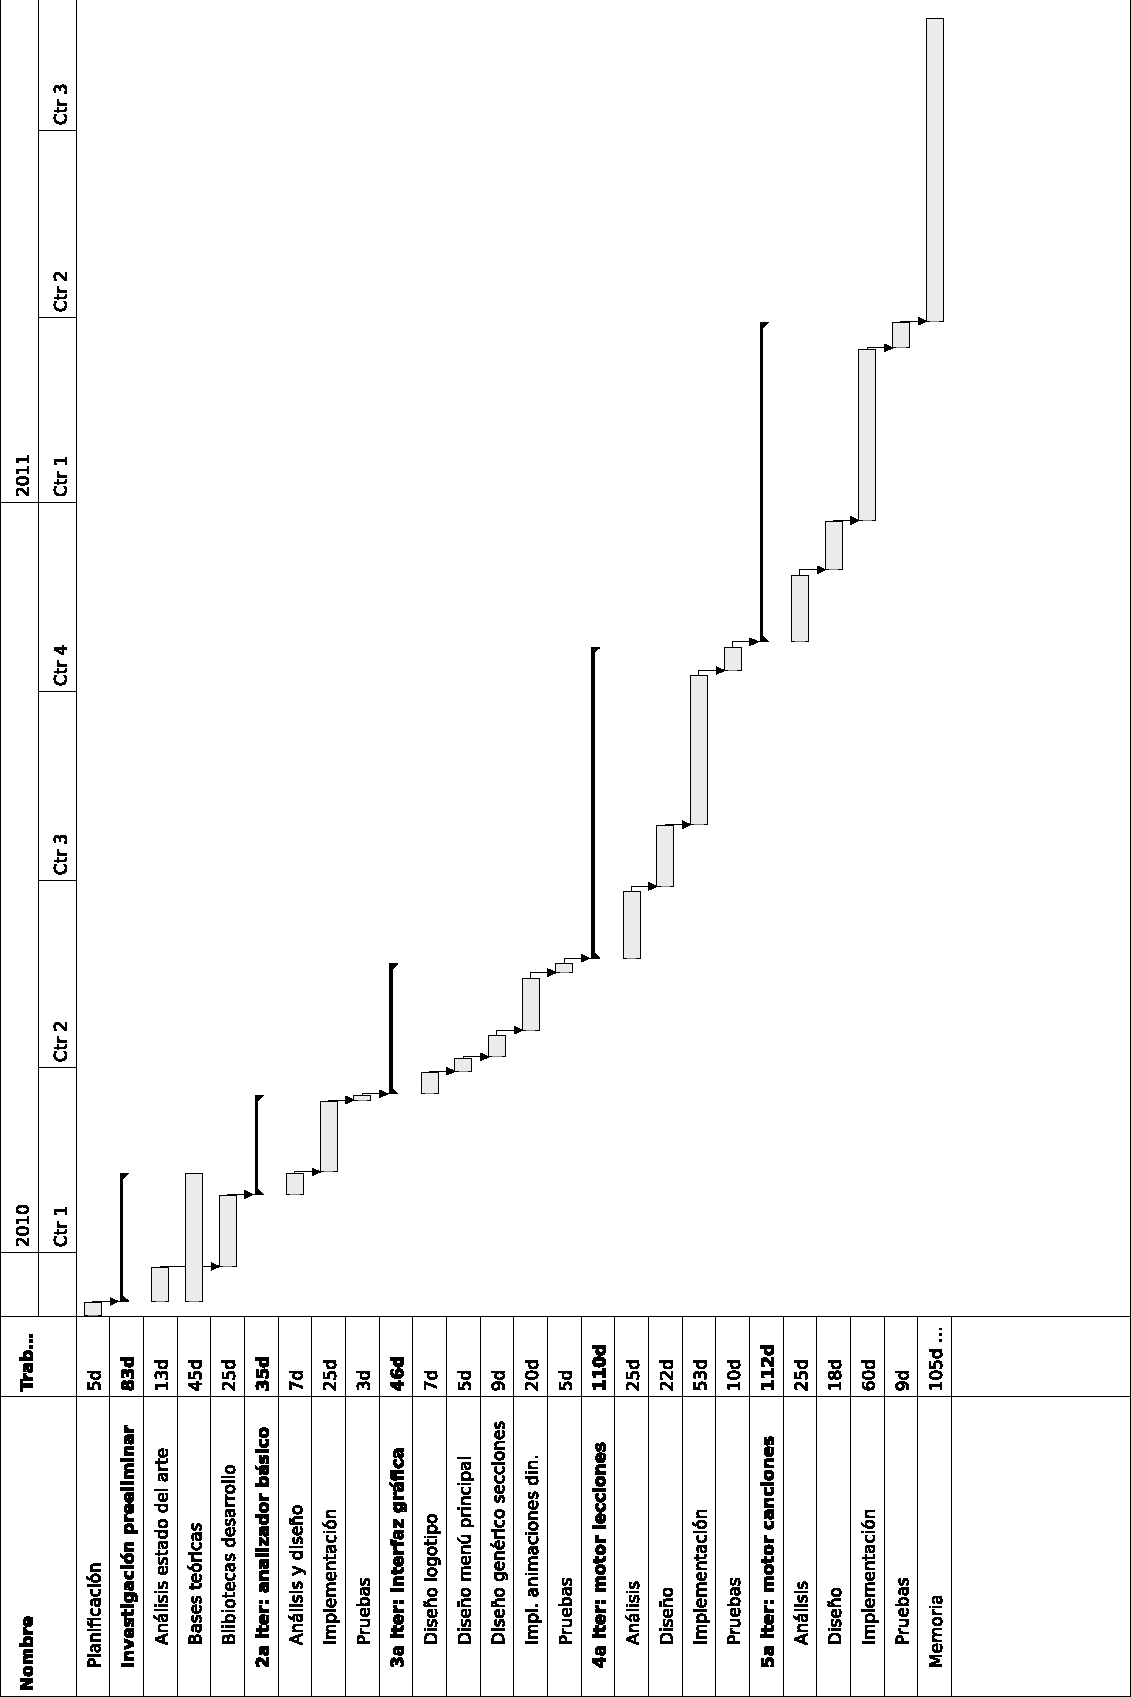
\includegraphics[width=0.95\textwidth]{imagen_diagrama_gantt}
  \caption{Diagrama Gantt de iteraciones}
  \label{fig:gantt}
\end{figure}


\section{Descripción general}
\textbf{oFlute} se modela como una herramienta lúdico-educativa para alumnos que
comiencen a aprender a usar la flauta dulce, proporcionando un entorno atractivo
y ameno para el estudiante. Éstos tendrán la posibilidad de comprobar sus
conocimientos sobre el uso de la flauta de forma totalmente práctica, gracias a
un motor de análisis del sonido capaz de detectar las notas que emite el jugador
con la flauta, capturadas por un micrófono, mediante el que la aplicación
valorará la pericia del estudiante con la flauta.

Además, los jugadores podrán recorrer una serie de pequeñas lecciones sobre
música en general, y el uso de la flauta dulce en particular. Estas lecciones
son totalmente ampliables, dando al usuario la posibilidad de crear las suyas
propias.

\subsection{Secciones de la aplicación}

\subsubsection{Análisis de notas}
Permite a los usuarios comprobar, de manera individual y pausada, que la
interpretación de cada una de las notas en la flauta es correcta. Para ello, se
presenta un pequeño analizador que responderá al sonido emitido por el usuario
con la flauta mostrando la nota tocada en pantalla.

\subsubsection{Motor de canciones}
Mediante este sistema, el usuario tendrá la oportunidad de interpretar canciones
completas a la vez que el computador analiza la eficacia del jugador,
otorgándole una puntuación en tiempo real. Además, el motor de canciones es
fácilmente expansible mediante ficheros de definición de canciones.

\subsubsection{Motor de lecciones}
Este sistema ofrece al usuario una serie de lecciones multimedia, con las que
podrá aprender sobre diferentes aspectos de la música en general y la flauta en
particular. Las lecciones cuentan con imágenes, texto y animaciones, que harán
que el aprendizaje sea entretenido y ameno. También es posible añadir nuevas
lecciones al sistema de forma sencilla.

\subsubsection{Calibración del micrófono}
\textbf{oFlute} ofrece la posibilidad de calibrar el micrófono, de forma que el
sistema se adapte al ruido ambiental y el análisis del sonido capturado sea lo
más exacto posible

\section{Implementación}
Durante el desarrollo del proyecto surgieron numerosas cuestiones y decisiones
de implementación. A continuación se presenta una selección de las que más
interés han generado. En la memoria del proyecto se desarrollan en mayor
extensión.

\subsection{Carga y uso de fuentes TrueType en Gosu}
La biblioteca principal utilizada en la implementación del proyecto es Gosu, una
librería de desarrollo de videojuegos 2D, multi-plataforma y con numerosas
características. Desafortunadamente, no era posible utilizar fuentes TrueType
cuando se utilizaba la biblioteca en GNU/Linux.

Utilizando los conocimientos de otra popular biblioteca, SDL, se consiguió
implementar un sistema para cargar y usar fuentes TrueType en Gosu de forma
eficiente. Esta implementación finalmente acabó formando parte oficial de la
biblioteca Gosu.

\subsection{Animaciones dinámicas}
Una de las decisiones iniciales de diseño fue la de hacer la interfaz gráfica de
usuario lo más atractiva posible, intentando utilizar gráficos amigables y, en
la medida de lo posible, animaciones y efectos dinámicos.

Con esto, se tornaba necesario crear un sistema de animaciones lo más versátil
posible, de forma que dotar a los elementos de la interfaz de movimiento fuera
un proceso sencillo. 



\section{Conclusiones y difusión}



\end{document}
